\begin{pastexam}[label={px:ccu-114-swa-04}]{中正資工所甲組 114 學年度 第 4 題}
（單選）

(5\%) (Choose \underline{one} best answer) Consider the red-black tree resulting from sequentially
inserting the following numbers into an empty red-black tree: 40, 60, 55, 15, 20, 5, 25, 30. What is the
sum of the numbers in the red nodes in the red-black tree?\\
(a)~145 \qquad (b)~125 \qquad (c)~110 \qquad (d)~90 \qquad (e)~None of the above.
\end{pastexam}

\begin{pastsoln}
答案是 (d) 90。

照資結書第~10.3.4~節的插入：新節點當紅色放到葉子；父節點紅時看叔叔，叔叔紅就把父、叔改黑、祖父改紅，
問題移到祖父；叔叔黑（含 \textsc{nil}）時，一直線就在祖父旋轉一次，折線就先在父節點旋轉成一直線，再在
祖父旋轉；旋轉上來的節點改黑、原祖父改紅。 最後根一律塗黑。 下面記號 $x$\textsuperscript{R}、
$x$\textsuperscript{B} 表示紅、黑，樹用「根（左子樹, 右子樹）」寫。

\begin{enumerate}
\item 插入 $40$：根，塗黑。 $40^{\mathrm{B}}$。
\item 插入 $60$：$40$ 的右子，紅；父黑，不用修正。
\item 插入 $55$：$60$ 的左子。 父 $60$ 紅、叔叔（$40$ 的左邊）\textsc{nil}；$55$ 是左子、$60$ 是右子，
折線。 先在 $60$ 右旋，再在 $40$ 左旋：$55^{\mathrm{B}}(40^{\mathrm{R}}, 60^{\mathrm{R}})$。
\item 插入 $15$：$40$ 的左子。 父 $40$ 紅、叔叔 $60$ 紅：$40$、$60$ 改黑，$55$ 改紅；$55$ 是根，塗回黑。
$55^{\mathrm{B}}(40^{\mathrm{B}}(15^{\mathrm{R}}, \cdot), 60^{\mathrm{B}})$。
\item 插入 $20$：$15$ 的右子。 父 $15$ 紅、叔叔（$40$ 的右邊）\textsc{nil}；折線。 先在 $15$ 左旋，再在
$40$ 右旋：$20$ 上來改黑，$15$、$40$ 是它的紅色子節點。 $55^{\mathrm{B}}(20^{\mathrm{B}}(15^{\mathrm{R}},
40^{\mathrm{R}}), 60^{\mathrm{B}})$。
\item 插入 $5$：$15$ 的左子。 父 $15$ 紅、叔叔 $40$ 紅：$15$、$40$ 改黑，$20$ 改紅；$20$ 的父 $55$ 黑，
結束。
\item 插入 $25$：$25 < 55$、$> 20$、$< 40$，放在 $40$ 的左子。 父 $40$ 黑，不用修正。
\item 插入 $30$：$30 > 25$，放在 $25$ 的右子。 父 $25$ 紅、叔叔（$40$ 的右邊）\textsc{nil}；$30$ 是右子、
$25$ 是左子，折線。 先在 $25$ 左旋，再在 $40$ 右旋：$30$ 上來改黑，$25$、$40$ 是它的紅色子節點。
\end{enumerate}

最後的樹（黑底白字是黑節點，淺紅底是紅節點）：
\begin{center}
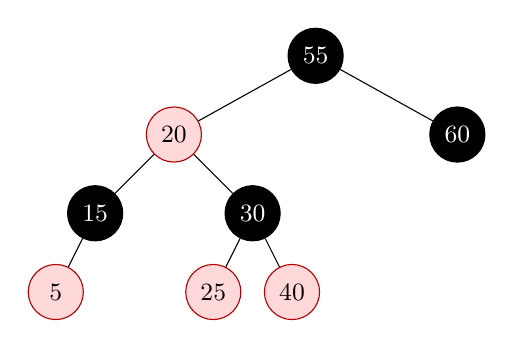
\begin{tikzpicture}[level distance=10mm,
  b/.style={circle,draw,fill=black,text=white,inner sep=1pt,minimum size=7mm,font=\small},
  r/.style={circle,draw=red!70!black,fill=red!15,inner sep=1pt,minimum size=7mm,font=\small},
  level 1/.style={sibling distance=36mm}, level 2/.style={sibling distance=20mm},
  level 3/.style={sibling distance=10mm}]
\node[b] {55}
  child {node[r] {20}
    child {node[b] {15} child {node[r] {5}} child[missing]}
    child {node[b] {30} child {node[r] {25}} child {node[r] {40}}}}
  child {node[b] {60}};
\end{tikzpicture}
\end{center}
檢查：根黑；沒有紅節點有紅子；每條根到 \textsc{nil} 的路徑都有 $2$ 個黑節點（不算 \textsc{nil}），例如
$55, 20, 15, 5$ 是 $55, 15$，$55, 60$ 是 $55, 60$。

紅節點是 $20, 5, 25, 40$，和為 $20 + 5 + 25 + 40 = 90$，選 (d)。
\end{pastsoln}
